\chapter{Introduction}\label{chap:introduction}
\section{What is Reinforcement Learning?}
\gls{rl} is an area of machine learning concerned with how intelligent agents ought to \bblue take actions in an environment \eblue 
in order to maximize some notion of cumulative reward. 
The agent learns to achieve a goal in an uncertain, potentially complex environment.
In \gls{rl}, an agent interacts with its environment, observes the state of the environment, and takes actions that affect the state. 
he agent also receives rewards from the environment. 
The agent's goal is to learn to act in a way that will maximize its expected cumulative reward over time.

\subsection{People and Connected Fields}
\begin{itemize}
\item Computer Science: Minsky, Barto, Sutton
\item Neuroscience:
\item Psychology: Holland, Klopf
\item Operations Research: Bertsekas, Puterman
\item Economics:
\item Engineering: Bellman, Tsitsiklis    
\end{itemize}

\begin{figure}[h!]
    \centering
    \resizebox{0.5\textwidth}{!}{%
    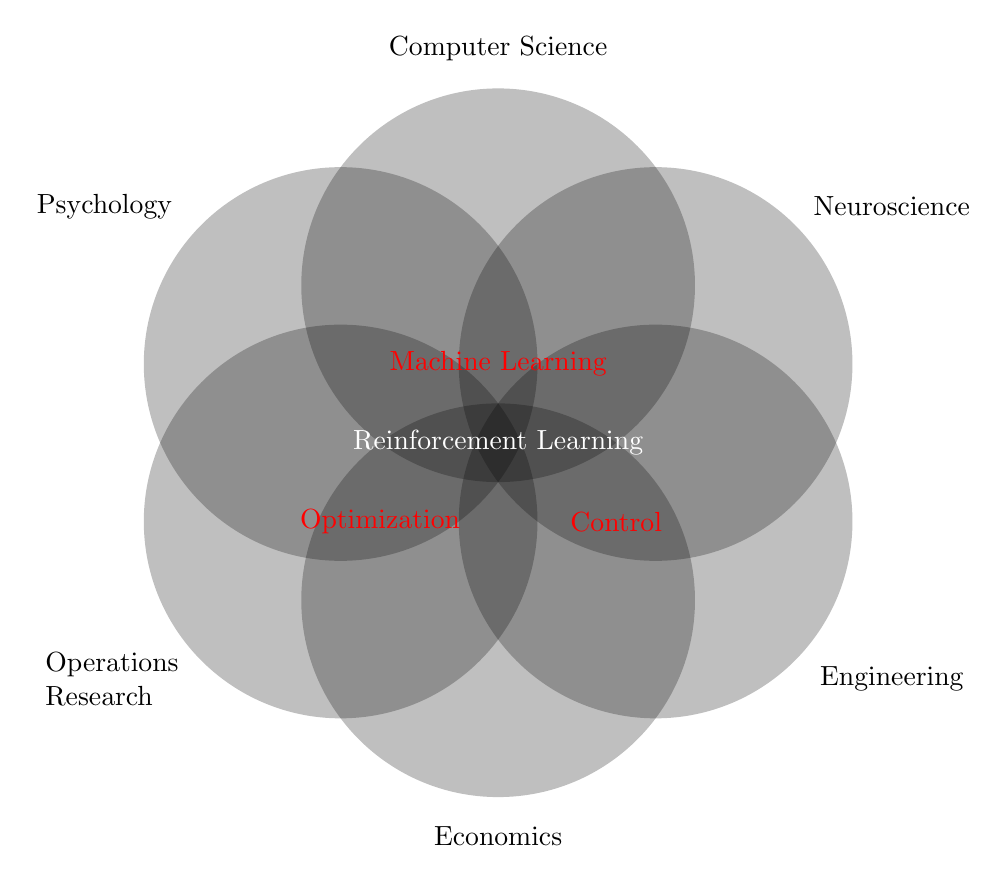
\begin{tikzpicture}
    \fill [nearly transparent](2,1) circle (2.5cm);
    \fill [nearly transparent](0,2) circle (2.5cm);
    \fill [nearly transparent](-2,1) circle (2.5cm);
    \fill [nearly transparent](-2,-1) circle (2.5cm);
    \fill [nearly transparent](0,-2) circle (2.5cm);
    \fill [nearly transparent](2,-1) circle (2.5cm);

    \node (cs) at (0,5) {Computer Science};
    \node (neuro) at (5,3) {Neuroscience};
    \node (psy) at (-5,3) {Psychology};
    \node [text width=1.5cm](or) at (-5,-3) {Operations Research};
    \node (eco) at (0,-5) {Economics};
    \node (eng) at (5,-3) {Engineering};
    \node[color = white] (rl) at (0,0) {Reinforcement Learning};
    \node[color = red] (oc) at (1.5,-1) {Control};
    \node[color = red] (opt) at (-1.5,-1) {Optimization};
    \node[color = red] (opt) at (0,1) {Machine Learning};

    \end{tikzpicture}
    }
    \caption{Reinforcement Learning}
    \label{fig:rl}
\end{figure}

\subsection{Mathematical Framework of Reinforcement Learning}

The basic building blocks of the mathematical formulation of


\subsection{Overview of Reinforcement Learning Approaches}
\begin{itemize}
\item \textbf{Value-based}
    \begin{itemize}
        \item Learns the optimal value function
        \item Example: Monte Carlo, SARSA, Q-learning, DQN
        \item \bred Low variance, not scalable to large action spaces \ered
    \end{itemize}
\item \textbf{Policy-based}
    \begin{itemize}
        \item Learns directly the optimal policy
        \item Example: Policy Gradient, NPG, TRPO, People
        \item \bred Scales to lathe and continuous action spaces, high variance \ered
    \end{itemize}
\item \textbf{Model-based}
    \begin{itemize}
        \item Learns bot the model \textit{P}, \textit{r} and the optimal Policy
        \item Example: Dyna, UCRL2, UCB-variance
        \item \bred Computationally expensive, but better sample efficiency \ered
    \end{itemize}
\end{itemize}

\begin{figure}
    \centering
    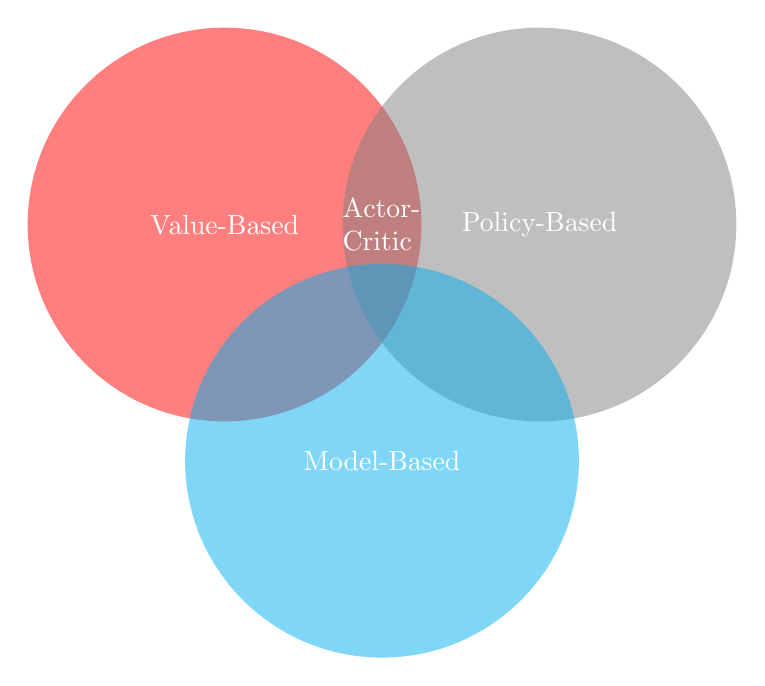
\begin{tikzpicture}

    \fill [color = red,semitransparent] (-2,1) circle (2.5cm);
    \fill [color = gray,semitransparent] (2,1) circle (2.5cm);
    \fill [color = cyan,semitransparent] (0,-2) circle (2.5cm);
    
    \node[color= white] (vb) at (-2,1) {Value-Based};
    \node[color= white] (pb) at (2,1) {Policy-Based};
    \node[color= white, text width = 1cm] (ac) at (0,1) {Actor-Critic};
    \node[color= white] (mb) at (0,-2) {Model-Based};
    \end{tikzpicture}
    \caption{Reinforcement Learning Approaches}
    \label{fig:rl-approaches}
\end{figure}
